\documentclass{article}


\usepackage[margin=0.6in]{geometry}
\usepackage{amssymb, amsmath, amsfonts}
\usepackage{mathtools}
\usepackage{physics}
\usepackage{placeins}
\usepackage{enumerate}
\usepackage{cancel}
\usepackage{array}
\usepackage{color}
\newcommand{\Rl}{\mathbb{R}}
\newcommand{\cov}{\text{cov}}
\newcommand{\vari}{\text{var}}
\newcommand{\cor}{\text{cor}}
\newcommand{\expec}{\mathbb{E}}
\newcommand{\f}[3]{#1\ :\ #2 \rightarrow #3}
\newcommand{\prob}[1]{\mathbb{P}\qty[#1]}

\title{PBG 200A Notes}
\author{Sam Fleischer}
\date{October 31, 2016}

\begin{document}
    \maketitle

    \section{Questions from the Notes}
        \subsubsection*{Question 1}
            \begin{align*}
                H_t &= H_0\exp(-\frac{t}{2N}) \\
                0.0049 &= 0.005\exp(-\frac{200/3}{2N}) \\
                \ln0.98 &= -\frac{200}{6N} \\
                N &= -\frac{200}{6\ln0.98} \\
                N &= 1650
            \end{align*}
        \subsubsection*{Question 2}
            $x = 0.5$:
            \begin{figure}[ht!]
                \centering
                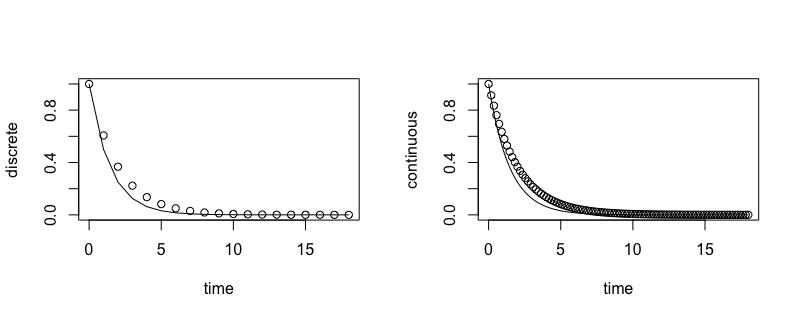
\includegraphics[scale=0.4]{fig1.png}\\
            \end{figure}
            \FloatBarrier
            $x = 0.1$:
            \begin{figure}[ht!]
                \centering
                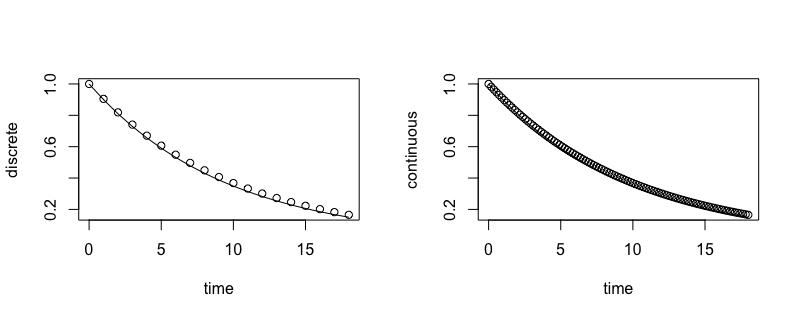
\includegraphics[scale=0.4]{fig2.png}\\
            \end{figure}
            \FloatBarrier
            $x = 0.01$:
            \begin{figure}[ht!]
                \centering
                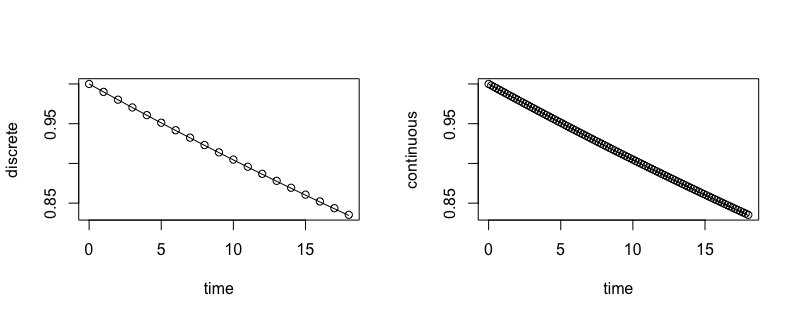
\includegraphics[scale=0.4]{fig3.png}\\
            \end{figure}
            \FloatBarrier

        \subsubsection*{Question 3}
            \begin{enumerate}[\bf\ \ A)]
                \item $\pi_1 = 0.0012$, $\pi_2 = 0.000014$ ?????
                \item $N_i = \frac{\theta_i}{4\mu}$ for $i = 1,2$.  If $\mu = 2\times10^{-8}$ and $\theta_1 = 0.0012$, then $N_1 = 15,000$.  If $\theta_2 = 0.000014$, then $N_2 = 175$.
                \item Oh my God they're adorable.
            \end{enumerate}

    \section{In-Class Notes}
        \subsection{Review}
            \begin{itemize}
                \item Neutral polymorphism/alleles
                \item Only $2\%$ encodes for proteins
                \item changes outside exons may by neutral if they do not disrupt regulatory sites
                \item examples of potentially neutral alleles:
                \begin{itemize}
                    \item synonymous changes in codons
                    \item non-synonymous changes which replaces one amino acid with a functionally similar one
                    \item non-synonymous change which produces a large change in a phenotype on which selection no longer acts
                \end{itemize}
            \end{itemize}
        \subsection{Loss of Heterozygosity}
            \begin{itemize}
                \item genetic drifts happens at a rate inversely proportional to population size (no genetic drift in infinite population size, i.e.~Hardy-Weinberg)
                \item
                \begin{align*}
                    H_t &= \qty(1 - \frac{1}{2N})\times H_{t-1} + \cancelto{0}{\frac{1}{2N}\times0} \\
                    H_t &= \qty(1 - \frac{1}{2N})^tH_0
                \end{align*}
                If $\frac{1}{2N} \ll 1$, then $1 - \frac{1}{2N} \approx \exp(-\frac{1}{2N})$, and thus $H_t \approx \exp(-\frac{t}{2N})H_0$.
            \end{itemize}
            \subsubsection{Examples}
                \begin{itemize}
                    \item the cheif of Pingelap island was heterozygous for colorblindness
                    \item Ashkenazi Jews and Tay-Sachs disease
                    \item extra fingers in Amish population
                \end{itemize}
        \subsection{Mutation can maintain nonzero equilibrium heterozygosity}
            We can write down the probability of no mutation between a pair of sequences,
            \begin{align*}
                \prob{\text{no mutation between sequences}} &= \frac{1}{2N}(1 - \mu)^2 + \frac{1}{2N}(1 - \frac{1}{2N})(1 - \mu)^4 + \frac{1}{2N}\qty(1 - \frac{1}{2N})^2\qty(1 - \mu)^6 \\
                &= \frac{1}{2N}\sum_{t=0}^\infty\qty[\qty(1-\frac{1}{2N})^t\qty(1 - \mu)^{2t+2}] \\
                &\approx \frac{1}{2N}\sum_{t=0}^\infty \exp[-\frac{t}{2N} - 2t\mu] \\
                &\approx \frac{1}{2N} \int_0^\infty \exp[-\frac{t}{2N} - 2t\mu]
            \end{align*}
            where $\mu$ is the rate of mutation and $N$ are the number of alleles.  This has a nice answer:
            \begin{align*}
                \prob{\text{no mutation between squences}} &= \frac{1}{2N}\qty(\frac{1}{\frac{1}{2N} + 2\mu}) = \frac{1}{1 + 4N\mu}
            \end{align*}
            Given that $4N\mu \ll 1$, we have $H = \dfrac{4N\mu}{1 + 4N\mu} \approx 4N\mu = \theta$.  The rate of genetic drift is slower in larger populations, so there is more of a chance for mutations to take hold.
        \subsection{Effective population size}
            The size of an ideal population $N_e$ in which drift occurs at the same rate as that in an actual population $N$:
            \begin{align*}
                N_e \ll N
            \end{align*}
            Bottlenecks so greatly affect the rate of loss of heterozygosity that the ``effective'' population size is close to the bottleneck sizes, not the large population size.  Harmonic mean is very sensitive to small numbers.
        \subsection{Coalescnce}
            We have
            \begin{align}
                t \sim \text{Geom}\qty(\frac{1}{2N}), \qquad \implies \qquad \expec[t] = 2N \text{ generations}
            \end{align}
            Often we assume $t \sim \text{Exp}\qty(\frac{1}{2N})$.  Given a mutation rate of $\mu$, then the number of mutations from two lineages going back $t$ generations is$ 2\mu t$, so
            \begin{align}
                \pi \coloneqq \expec[\text{pairwise diferences}] = 2\mu\expec[t] = 2\mu2N = 4N\mu = \theta
            \end{align}
            $\pi$ is the observation - $\theta$ is the theoretical value.

\end{document}















